\documentclass[12pt]{article}
%% \documentclass[twocolumn]{} : separa o documento em duas colunas
%% 
%%

%%&&&&&&&&&&&&&
%%	PACOTES  &&
%%&&&&&&&&&&&&&

\usepackage[utf8]{inputenc} %Este pacote adciona suporte acentuação
\usepackage[brazil]{babel} %Este pacote traduz comandos para pt-br
\usepackage{indentfirst} %Este pacote identa primeiro parágrafo
\usepackage{setspace} %Este pacote altera espaçamento entre linhas
\usepackage[a4paper, left=1cm, right=2cm, top=2cm, bottom=3cm]{geometry} %Este pacote altera margem do documento
\usepackage[usenames, dvipsnames]{xcolor} %Modifica as cores [pacotes adcionais de cores]
\usepackage{graphicx} %Este pacote adciona suporte a figuras
\usepackage{float} %Este pacote força posicionamento de figuras
\usepackage{subcaption} %Este pacote adciona suporte subfiguras
\usepackage{wrapfig} %Este pacote permite colocar figura no meio do texto
\usepackage{multirow} %Este pacote adciona suporte mesclagem linhas
\usepackage{tabularx} %Este pacote permite personalizaçao margens da tabela
\usepackage{amsmath} %Este pacote inclui modo matemático
\usepackage{natbib} %Este pacote adciona opções de citações
\usepackage{multicol} %Este pacote adciona colunas personalizadas
\usepackage[perpage]{footmisc} %Este pacote reseta contagem de rodapé por página
\usepackage{csquotes} 

%%&&&&&&&&&&&&&&&&
%%	PARÂMETROS  &&
%%&&&&&&&&&&&&&&&&

%%
%%  PARÁGRAFO
%%
\setlength{\parindent}{1.5cm} %Comando altera identação dos parágrafos
\setlength{\parskip}{1cm} %Comando altera espaçamentos entre parágrafos

%%
%%	COLUNAS
%%
\setlength{\columnsep}{5mm} %distância entre colunas
\setlength{\columnseprule}{0.5mm} %adciona separador entre colunas

%% Redefinição de comandos matemáticos
%%
\renewcommand{\sin}{\mathrm{ sen\hspace{0.5mm} }}
\renewcommand{\tan}{\mathrm{ tg\hspace{0.5mm} }}

%% Redefinição de contador de rodapé
%%
\renewcommand{\thefootnote}{\roman{footnote}} %muda estilo de contagem para algarismo romano

%Cores personalizadas
\definecolor{minhacorrgb}{RGB}{85,158,131} %define cor personalizada

%%&&&&&&&&&&&&&%%
%%	DOCUMENTO  &&
%%&&&&&&&&&&&&&%%

\begin{document}
	%%
	%%	ESTUDO CAPA
	\title{ \textbf{ESTUDO DE LATEX} } %cria título
	\author{ \textit{Helio M. Andrade Jr.} } %cria autor
	\date{11 de abril de 2019} %cria data
	\maketitle %gera título baseado nos parâmetros acima
	%%
	%% ESTUDO NUMERAÇÃO PÁGINA
	\thispagestyle{empty} %Oculta numeração de páginas
	\newpage
	
	
	%%
	%%	ESTUDO CONTENT
	
	%%%
	\setcounter{page}{1} %reseta contagem de páginas
	\pagenumbering{roman} %altera numeração página para algorismo romano (para maiúsculo usar Roman)
	
	\tableofcontents %cria sumário
	\newpage
	
	\listoffigures %cria sumário de figuras
	\newpage
	
	\listoftables %cria sumário de tabelas
	\newpage
	
	%%
	%% 	ESTUDO SEÇÕES
	%%
	\setcounter{page}{1}  %reseta contagem de páginas (boa prática deixar explícito)
	\pagenumbering{arabic} %altera numeração página para algorismo arábico
	\section{Título grand\~ao}
		Ac turpis egestas sed tempus urna et pharetra pharetra. Sit amet nisl purus in. At quis risus sed vulputate odio ut. Placerat duis ultricies lacus sed turpis tincidunt id aliquet. Quis vel eros donec ac odio tempor orci dapibus. Sit amet mattis vulputate enim nulla aliquet porttitor lacus luctus. Ornare suspendisse sed nisi lacus sed viverra tellus. Aliquet nibh praesent tristique magna sit amet purus gravida. Risus at ultrices mi tempus. Eu sem integer vitae justo eget magna. Diam ut venenatis tellus in metus vulputate eu scelerisque felis. Nunc sed augue lacus viverra vitae. Quis eleifend quam adipiscing vitae proin. Ante in nibh mauris cursus mattis. Scelerisque in dictum non consectetur a erat nam. Senectus et netus et malesuada fames ac turpis egestas. Id faucibus nisl tincidunt eget nullam. Scelerisque viverra mauris in aliquam sem fringilla ut.
		\subsection{Título subseção}
		\label{subsec:tit_subsec}
			Volutpat commodo sed egestas egestas fringilla phasellus. Sit amet nisl suscipit adipiscing bibendum est ultricies integer. Blandit libero volutpat sed cras ornare arcu dui vivamus arcu. Facilisis gravida neque convallis a cras semper. Venenatis a condimentum vitae sapien pellentesque habitant. Proin nibh nisl condimentum id venenatis a condimentum. Aliquam sem et tortor consequat id porta nibh. Semper feugiat nibh sed pulvinar. Mi eget mauris pharetra et. Placerat vestibulum lectus mauris ultrices eros in. Egestas egestas fringilla phasellus faucibus scelerisque eleifend donec pretium vulputate. Convallis aenean et tortor at risus. Aliquet bibendum enim facilisis gravida neque convallis a. Pharetra massa massa ultricies mi quis hendrerit dolor magna. Sapien et ligula ullamcorper malesuada proin.
		\subsubsection{Título de subsubseção}
			Lorem ipsum dolor sit amet, consectetur adipiscing elit, sed do eiusmod tempor incididunt ut labore et dolore magna aliqua. Ut enim ad minim veniam, quis nostrud exercitation ullamco laboris nisi ut aliquip ex ea commodo consequat. Duis aute irure dolor in reprehenderit in voluptate velit esse cillum dolore eu fugiat nulla pariatur. Excepteur sint occaecat cupidatat non proident, sunt in culpa qui officia deserunt mollit anim id est laborum.
			
			%Espaço cria novo parágrafo
			Lorem ipsum dolor sit amet, consectetur adipiscing elit, sed do eiusmod tempor incididunt ut labore et dolore magna aliqua. Ut enim ad minim veniam, quis nostrud exercitation ullamco laboris nisi ut aliquip ex ea commodo consequat. Duis aute irure dolor in reprehenderit in voluptate velit esse cillum dolore eu fugiat nulla pariatur. Excepteur sint occaecat cupidatat non proident, sunt in culpa qui officia deserunt mollit anim id est laborum.
		\newpage %quebra página

	%%
	%%	ESTUDO FORMATAÇÃO TEXTO
	%%
	\textbf{Texto em negrito}
	
	{\em Texto em ênfase switch em}
	
	\textit{Texto em itálico}
	
	\underline{Texto sublinhado}
	
	\begin{flushright}
		Texto à direita
	\end{flushright}
	
	\begin{center}
		Texto centralizado
	\end{center}
	
	\begin{flushleft}
		Texto à esquerda
	\end{flushleft}
	
	\begin{tiny}
		texto pequeno
	\end{tiny}
	
	Texto normal
	
	{\Huge TEXTO GIGANTE}
	
	\newpage
	
	%%
	%%	ESTUDO PARÁGRAFOS
	%%
	\section{Seção espaçamento linhas}
		\doublespacing %Espaçamento duplo entre linhas (até o final do documento)
		Ac turpis egestas sed tempus urna et pharetra pharetra. Sit amet nisl purus in. At quis risus sed vulputate odio ut. Placerat duis ultricies lacus sed turpis tincidunt id aliquet. Quis vel eros donec ac odio tempor orci dapibus. Sit amet mattis vulputate enim nulla aliquet porttitor lacus luctus. Ornare suspendisse sed nisi lacus sed viverra tellus. Aliquet nibh praesent tristique magna sit amet purus gravida. Risus at ultrices mi tempus. Eu sem integer vitae justo eget magna. Diam ut venenatis tellus in metus vulputate eu scelerisque felis. Nunc sed augue lacus viverra vitae. Quis eleifend quam adipiscing vitae proin. Ante in nibh mauris cursus mattis. Scelerisque in dictum non consectetur a erat nam. Senectus et netus et malesuada fames ac turpis egestas. Id faucibus nisl tincidunt eget nullam. Scelerisque viverra mauris in aliquam sem fringilla ut.
		
		\begin{onehalfspace} %modifica espaçamento entre linha de um parágrafo específico
			Urna duis convallis convallis tellus id. Eget felis eget nunc lobortis mattis aliquam. Eget felis eget nunc lobortis mattis aliquam. Auctor augue mauris augue neque gravida in fermentum. Aliquam sem et tortor consequat id porta nibh venenatis. Lobortis scelerisque fermentum dui faucibus in ornare quam viverra. Urna nunc id cursus metus aliquam eleifend mi. Sit amet tellus cras adipiscing enim eu turpis. Amet consectetur adipiscing elit pellentesque. Consequat nisl vel pretium lectus quam id leo in vitae.
		\end{onehalfspace}
	
		\setstretch{2.5} %Espaçamento personalizado entre linhas
		Libero volutpat sed cras ornare arcu dui vivamus. Pharetra convallis posuere morbi leo urna molestie. Quis imperdiet massa tincidunt nunc pulvinar sapien. Purus faucibus ornare suspendisse sed nisi. In dictum non consectetur a erat nam. Imperdiet sed euismod nisi porta lorem mollis aliquam ut porttitor. Varius quam quisque id diam vel quam. Facilisis sed odio morbi quis commodo odio aenean. Ornare arcu odio ut sem nulla. Dictumst quisque sagittis purus sit amet volutpat. Nulla posuere sollicitudin aliquam ultrices.
			
		\begin{spacing}{0.5} %Espaçamento perosnalizado entre linhas usando begin|end
			Pretium viverra suspendisse potenti nullam ac tortor vitae. Duis at consectetur lorem donec massa. Massa tincidunt nunc pulvinar sapien et ligula. Risus in hendrerit gravida rutrum quisque non tellus orci ac. Risus quis varius quam quisque id diam vel quam elementum. At tempor commodo ullamcorper a lacus vestibulum. Interdum velit euismod in pellentesque massa placerat. Feugiat in ante metus dictum at tempor commodo ullamcorper. Sodales ut eu sem integer vitae justo. Magna sit amet purus gravida quis blandit turpis. Porta lorem mollis aliquam ut porttitor leo a diam. Mus mauris vitae ultricies leo integer malesuada. At in tellus integer feugiat. Malesuada fames ac turpis egestas sed tempus urna et pharetra.
		\end{spacing}
		
		\singlespacing %Espaçamento padrão entre linhas (a partir daqui)
	\subsection{Subsecão Horizontal Space}
		\hspace{0cm}Lorem ipsum dolor sit amet, consectetur adipiscing elit, sed do eiusmod tempor incididunt ut labore et dolore magna aliqua. Mi quis hendrerit dolor magna eget est lorem ipsum. %altera o espaço HORIZONTAL do parágrafo somado ao padrão
		\hspace{1cm}Sagittis id consectetur purus ut. Iaculis nunc sed augue lacus viverra vitae congue. Adipiscing elit ut aliquam purus. Metus aliquam eleifend mi in nulla posuere. 
		\hspace{2cm}Amet purus gravida quis blandit. Vel eros donec ac odio tempor orci. Vitae nunc sed velit dignissim sodales ut. Nisl tincidunt eget nullam non.
		
	\subsubsection{Subsubseção Vertical Space}
		\vspace{1.5cm} %altera espaço VERTICAL entre parágrafos somado ao padrão
		Volutpat commodo sed egestas egestas fringilla phasellus. Sit amet nisl suscipit adipiscing bibendum est ultricies integer. Blandit libero volutpat sed cras ornare arcu dui vivamus arcu. Facilisis gravida neque convallis a cras semper. Venenatis a condimentum vitae sapien pellentesque habitant. Proin nibh nisl condimentum id venenatis a condimentum. Aliquam sem et tortor consequat id porta nibh. Semper feugiat nibh sed pulvinar. Mi eget mauris pharetra et. \vspace{1cm}Placerat vestibulum lectus mauris ultrices eros in. Egestas egestas fringilla phasellus faucibus scelerisque eleifend donec pretium vulputate. Convallis aenean et tortor at risus. Aliquet bibendum enim facilisis gravida neque convallis a. Pharetra massa massa ultricies mi quis hendrerit dolor magna. Sapien et ligula ullamcorper malesuada proin.
	\newpage	
	
	%%
	%%	ESTUDO CORES
	%%
	\section{Seção cores}
	\pagecolor{yellow} %muda cor das páginas da atual em diante
	\textcolor{red}{Textarium em vermelhus. Ac turpis egestas sed tempus urna et pharetra pharetra. Sit amet nisl purus in. At quis risus sed vulputate odio ut. Placerat duis ultricies lacus sed turpis tincidunt id aliquet. Quis vel eros donec ac odio tempor orci dapibus. Sit amet mattis vulputate enim nulla aliquet porttitor lacus luctus. Ornare suspendisse sed nisi lacus sed viverra tellus. Aliquet nibh praesent tristique magna sit amet purus gravida.} 
	
	\begin{flushleft}
		\colorbox{SkyBlue}{ %caixa de cor
			\parbox{\textwidth}{%cria caia  {define largura da caixa igual largura do corpo do texto}
				at ultrices mi tempus. Eu sem integer vitae justo eget magna. Diam ut venenatis tellus in metus vulputate eu scelerisque felis. Nunc sed augue lacus viverra vitae. Quis eleifend quam adipiscing vitae proin. Ante in nibh mauris cursus mattis. Scelerisque in dictum non consectetur a erat nam. Senectus et netus et malesuada fames ac turpis egestas. Id faucibus nisl tincidunt eget nullam. Scelerisque viverra mauris in aliquam sem fringilla ut.} }
	\end{flushleft}
	
	
	\newpage
	
	Libero volutpat sed cras ornare arcu dui vivamus. Pharetra convallis posuere morbi leo urna molestie. Quis imperdiet massa tincidunt nunc pulvinar sapien. Purus faucibus ornare suspendisse sed nisi. In dictum non consectetur a erat nam. Imperdiet sed euismod nisi porta lorem mollis aliquam ut porttitor. Varius quam quisque id diam vel quam. Facilisis sed odio morbi quis commodo odio aenean. Ornare arcu odio ut sem nulla. Dictumst quisque sagittis purus sit amet volutpat. Nulla posuere sollicitudin aliquam ultrices.
	
	Pretium viverra suspendisse potenti nullam ac tortor vitae. Duis at consectetur lorem donec massa. Massa tincidunt nunc pulvinar sapien et ligula. Risus in hendrerit gravida rutrum quisque non tellus orci ac. Risus quis varius quam quisque id diam vel quam elementum. At tempor commodo ullamcorper a lacus vestibulum. Interdum velit euismod in pellentesque massa placerat. Feugiat in ante metus dictum at tempor commodo ullamcorper. Sodales ut eu sem integer vitae justo. Magna sit amet purus gravida quis blandit turpis. Porta lorem mollis aliquam ut porttitor leo a diam. Mus mauris vitae ultricies leo integer malesuada. At in tellus integer feugiat. Malesuada fames ac turpis egestas sed tempus urna et pharetra.
	
	\newpage
	%%
	%%	ESTUDO LISTAS
	%%
	\pagecolor{white} %muda cor da página para branco
	\section{Seção de listas}
		Ac turpis egestas sed tempus urna et pharetra pharetra. Sit amet nisl purus in. At quis risus sed vulputate odio ut. Placerat duis ultricies lacus sed turpis tincidunt id aliquet. Quis vel eros donec ac odio tempor orci dapibus. Sit amet mattis vulputate enim nulla aliquet porttitor lacus luctus. 
		
		Lista não-ordenada:
		\begin{itemize} % Lista não enumerada
			\item Primeiro item
			\item Segundo item
				\begin{itemize}
					\item primeiro sub item
					\item segundo sub item
						\begin{itemize}
							\item sub sub item
						\end{itemize}
				\end{itemize}
			\item Terceiro item
		\end{itemize}
		
		Lista ordenada:
		\begin{enumerate}
			\item Numerado um
				\begin{enumerate}
					\item Subnumerado 1
						\begin{itemize}
							\item Item qualquer aí
						\end{itemize}
					\item Sumnumerado 2
				\end{enumerate}
			\item Numerado dois
			\item Numerado três
		\end{enumerate}
	
		Lista descritiva:
		\begin{description}
			\item[PRIMEIRO] fala alguma coisa sobre o primeiro item
			\item[SEGUNDO] fala alguma coisa sobre o segundo item
				\begin{description}
					\item[Subitem descritivo] mais descrição aqui, eta carai.
				\end{description}
		\end{description}
	\newpage
	
	%%
	%%	Estudos Figuras
	%%
	\section{Seção Figuras}
		Lorem ipsum dolor sit amet, consectetur adipiscing elit, sed do eiusmod tempor incididunt ut labore et dolore magna aliqua. Massa eget egestas purus viverra accumsan in nisl. A condimentum vitae sapien pellentesque habitant morbi. Erat velit scelerisque in dictum non consectetur. Fringilla urna porttitor rhoncus dolor purus non enim praesent. Id diam maecenas ultricies mi eget mauris pharetra et ultrices. Posuere urna nec tincidunt praesent semper feugiat nibh sed. Nibh tellus molestie nunc non blandit. Aliquam id diam maecenas ultricies mi eget. Consectetur libero id faucibus nisl. Metus dictum at tempor commodo ullamcorper. Fringilla urna porttitor rhoncus dolor. Morbi leo urna molestie at elementum. Eu consequat ac felis donec et. Quis imperdiet massa tincidunt nunc pulvinar sapien et ligula. Nunc mi ipsum faucibus vitae aliquet nec.
		
		\begin{figure}[H] % [H] coloca imagem em posição precisamente igual no código
			\centering
			
\includegraphics[width=0.7\linewidth]{figuras/birb_01}
			\caption[Legenda curta do birb trabalhador]{Legenda longa do birb trabalhador}
			\label{fig:birb01}
		\end{figure}

		Ipsum dolor sit amet consectetur adipiscing elit. Elementum tempus egestas sed sed risus. Proin nibh nisl condimentum id venenatis a condimentum vitae. Massa enim nec dui nunc mattis enim ut tellus. In est ante in nibh mauris cursus. Dignissim cras tincidunt lobortis feugiat. Cras semper auctor neque vitae. Metus dictum at tempor commodo. Sit amet est placerat in egestas erat imperdiet sed euismod. Ultrices tincidunt arcu non sodales neque sodales ut. Consequat interdum varius sit amet mattis vulputate enim. Metus aliquam eleifend mi in nulla posuere. Consequat interdum varius sit amet mattis vulputate enim nulla aliquet. Non pulvinar neque laoreet suspendisse interdum consectetur libero. Lectus urna duis convallis convallis tellus. Morbi tristique senectus et netus et malesuada fames. Purus faucibus ornare suspendisse sed nisi lacus sed viverra. At ultrices mi tempus imperdiet. Sit amet mauris commodo quis imperdiet massa tincidunt nunc pulvinar. Egestas pretium aenean pharetra magna ac placerat.
		
		%Figuras com subfiguras
		\begin{figure}[H]
			\centering
			\caption[Legenda curta do birb BIRL]{Legenda longa do birb BIRL}
			\begin{subfigure}[b]{0.3\textwidth}
				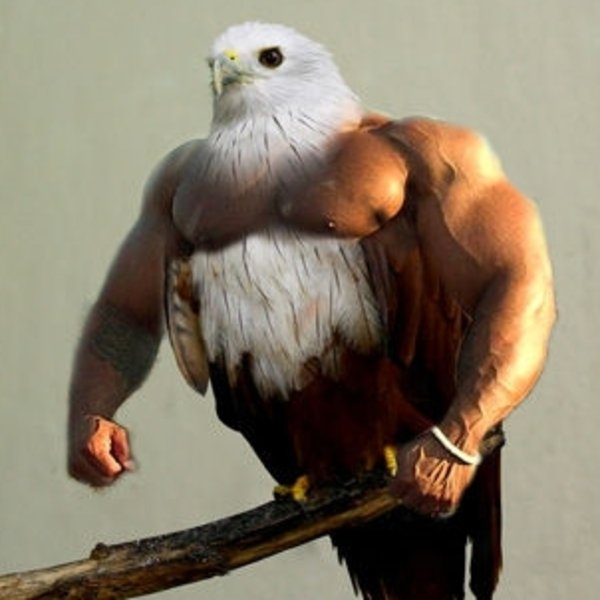
\includegraphics[width=\linewidth]{figuras/birb_02a}
				\caption{Birl hawk}
				\label{fig:birlhawk}
			\end{subfigure}
			~ %adciona espaço entre as figuras na linha
			\begin{subfigure}[b]{0.3\textwidth}
				
\includegraphics[width=\linewidth]{figuras/birb_02b}
				\caption{Birl owl}
				\label{fig:birlowl}
			\end{subfigure}
			\quad
			\begin{subfigure}[b]{0.3\textwidth}
				
\includegraphics[width=\linewidth]{figuras/birb_02c}
				\caption{Birl chicken}
				\label{fig:birlchicken}
			\end{subfigure}
			\label{fig:birb02}
		\end{figure}
	
		Lectus arcu bibendum at varius vel pharetra vel turpis nunc. Malesuada fames ac turpis egestas. Faucibus scelerisque eleifend donec pretium vulputate sapien nec. Magna sit amet purus gravida quis blandit. Orci nulla pellentesque dignissim enim sit amet venenatis urna cursus. Arcu non sodales neque sodales ut etiam sit amet. Velit laoreet id donec ultrices. Morbi tristique senectus et netus et malesuada fames ac turpis. Nunc sed augue lacus viverra vitae congue eu consequat. Justo eget magna fermentum iaculis eu non. Ridiculus mus mauris vitae ultricies. Tellus in hac habitasse platea dictumst vestibulum rhoncus est pellentesque. Morbi enim nunc faucibus a pellentesque sit amet porttitor. Ut venenatis tellus in metus vulputate eu scelerisque. Viverra maecenas accumsan lacus vel facilisis. Blandit libero volutpat sed cras ornare arcu. Rutrum tellus pellentesque eu tincidunt tortor aliquam nulla. Sollicitudin nibh sit amet commodo nulla facilisi nullam vehicula. Sollicitudin nibh sit amet commodo nulla facilisi nullam vehicula. Lectus quam id leo in vitae turpis massa sed elementum.
		\newpage
		
		\begin{wrapfigure}{r}{0.5\textwidth}
			\vspace{-10pt}
			\begin{center}
				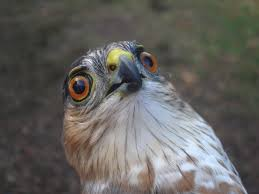
\includegraphics[width=0.48\textwidth]{figuras/birb_03}
			\end{center}
			\vspace{-20pt} %Diminui espaço entre legenda e imagem
			\caption[Legenda curta do birb puto]{Legenda longa do birb puto}
			\vspace{-10pt} %Diminiui espaço vertical entre legenda e texto
			\label{fig:birb03}
		\end{wrapfigure}
	
		Turpis egestas pretium aenean pharetra magna ac placerat. Sed adipiscing diam donec adipiscing tristique risus nec. Aliquam eleifend mi in nulla posuere sollicitudin aliquam. Sagittis eu volutpat odio facilisis mauris sit. Faucibus vitae aliquet nec ullamcorper sit amet risus. Egestas maecenas pharetra convallis posuere morbi leo. Elementum tempus egestas sed sed risus pretium quam vulputate dignissim. Aliquet eget sit amet tellus cras adipiscing enim eu turpis. Malesuada fames ac turpis egestas integer eget aliquet nibh. Sed risus ultricies tristique nulla aliquet. Adipiscing commodo elit at imperdiet dui accumsan. Orci phasellus egestas tellus rutrum tellus pellentesque. Ultricies mi quis hendrerit dolor. Vehicula ipsum a arcu cursus. Arcu bibendum at varius vel pharetra vel. Et tortor at risus viverra adipiscing at in tellus integer. Tincidunt tortor aliquam nulla facilisi cras fermentum odio. Tortor condimentum lacinia quis vel eros donec ac odio tempor.
		\newpage
		
		%%
		%%	ESTUDO TABELAS
		%%
		\section{Seção das tabelas}
			Orci a scelerisque purus semper eget duis at tellus at. Molestie at elementum eu facilisis sed. Adipiscing tristique risus nec feugiat in fermentum posuere urna. A condimentum vitae sapien pellentesque habitant morbi tristique senectus et. Etiam erat velit scelerisque in dictum non. Arcu cursus vitae congue mauris rhoncus aenean. Sed augue lacus viverra vitae congue eu consequat. Pellentesque pulvinar pellentesque habitant morbi tristique senectus et netus et. Hendrerit gravida rutrum quisque non. Et netus et malesuada fames ac turpis egestas maecenas. Id cursus metus aliquam eleifend mi in. Dapibus ultrices in iaculis nunc sed augue lacus viverra vitae.
			
			\begin{table}[H]
				\centering
				\caption[Legenda curta da tabela]{Legenda longa da tabela}
				\label{tab:tab1}
				\begin{tabular}{ l|l|l } % | reprensa as bordas verticais, l (alinhando a esquerda)
					%\hline %linha horizontal
					A1 & B1 & C1 \\ \hline 
					A2 & B2 & C2 \\ \hline
					A3 & B3 & C3 \\ %\hline
				\end{tabular}
				\vspace{-30pt}
			\end{table}
		
			Pellentesque elit ullamcorper dignissim cras tincidunt. Sit amet volutpat consequat mauris nunc. Odio eu feugiat pretium nibh. Morbi tincidunt augue interdum velit euismod in pellentesque massa placerat. Elementum sagittis vitae et leo. Massa massa ultricies mi quis hendrerit dolor magna. Scelerisque purus semper eget duis at. Phasellus egestas tellus rutrum tellus pellentesque eu tincidunt. Diam vel quam elementum pulvinar. Tincidunt arcu non sodales neque sodales ut etiam. Id neque aliquam vestibulum morbi blandit cursus risus at ultrices. Id porta nibh venenatis cras. Ullamcorper malesuada proin libero nunc. Malesuada fames ac turpis egestas sed tempus urna et. Ultricies mi quis hendrerit dolor magna eget est. Odio aenean sed adipiscing diam donec adipiscing tristique. Egestas pretium aenean pharetra magna ac placerat vestibulum. Nulla facilisi nullam vehicula ipsum a arcu cursus vitae.
			
			\begin{table}[H] %H define 
				\centering
				\caption[Legenda curta da tabela 2]{Legenda longa da tabela 2}
				\label{tab:tab2}
				\begin{tabular}{|l|l|l|}
					\hline
					A1 & \multicolumn{2}{l|}{B1} \\ \hline %comando multicolumn para especificar quantas células mesclar {coluna}{Align |(borda)}{conteúdo}
					A2 & B2         & C2         \\ \hline
					A3 & B3         & C3         \\ \hline
				\end{tabular}
			\end{table}
			
			Lorem ipsum dolor sit amet, consectetur adipiscing elit, sed do eiusmod tempor incididunt ut labore et dolore magna aliqua. Massa eget egestas purus viverra accumsan in nisl. A condimentum vitae sapien pellentesque habitant morbi. Erat velit scelerisque in dictum non consectetur. Fringilla urna porttitor rhoncus dolor purus non enim praesent. Id diam maecenas ultricies mi eget mauris pharetra et ultrices. Posuere urna nec tincidunt praesent semper feugiat nibh sed. Nibh tellus molestie nunc non blandit. Aliquam id diam maecenas ultricies mi eget. Consectetur libero id faucibus nisl. Metus dictum at tempor commodo ullamcorper. Fringilla urna porttitor rhoncus dolor. Morbi leo urna molestie at elementum. Eu consequat ac felis donec et. Quis imperdiet massa tincidunt nunc pulvinar sapien et ligula. Nunc mi ipsum faucibus vitae aliquet nec.

			\renewcommand{\arraystretch}{3} %altera as margens verticais das tabelas a partir daqui
			\begin{table}[H]
				\centering
				\caption[Legenda curta da tabela 3]{Legenda longa da tabela 3}
				\label{tab:tab3}
				\begin{tabularx}{0.5\textwidth}{|X|X|X|} % X indica quais colunas devem ser expandidas
					\hline
					\centering A1 & \multicolumn{2}{c|} %multicolumn mesclagem de colunas ; {c|} centraliza o texto {\multirow{2}{*}{B1}}
									 {\multirow{2}{*}{B1}} %multirow define númeno de linhas para mesclar
									 \\ \cline{1-1} %indica de que célula até qual célula a borda vai
					\hfill A2 & \multicolumn{2}{l|}{}                    \\ \hline %hfill alinha a direita
					A3 & B3                  & C3                 \\ \hline
				\end{tabularx}
				\vspace{-20pt}
			\end{table}
			\renewcommand{\arraystretch}{1}
			
			Ipsum dolor sit amet consectetur adipiscing elit. Elementum tempus egestas sed sed risus. Proin nibh nisl condimentum id venenatis a condimentum vitae. Massa enim nec dui nunc mattis enim ut tellus. In est ante in nibh mauris cursus. Dignissim cras tincidunt lobortis feugiat. Cras semper auctor neque vitae. Metus dictum at tempor commodo. Sit amet est placerat in egestas erat imperdiet sed euismod. Ultrices tincidunt arcu non sodales neque sodales ut. Consequat interdum varius sit amet mattis vulputate enim. Metus aliquam eleifend mi in nulla posuere. Consequat interdum varius sit amet mattis vulputate enim nulla aliquet. Non pulvinar neque laoreet suspendisse interdum consectetur libero. Lectus urna duis convallis convallis tellus. Morbi tristique senectus et netus et malesuada fames. Purus faucibus ornare suspendisse sed nisi lacus sed viverra. At ultrices mi tempus imperdiet. Sit amet mauris commodo quis imperdiet massa tincidunt nunc pulvinar. Egestas pretium aenean pharetra magna ac placerat.
			\newpage
			
			%%
			%%	SEÇÃO MATEMÁTICA
			%%
			
			\section{Seção matemática}
			%%ESTUDO DE EQUAÇÕES
			%%
			\subsection{Ambiente de equações}
				Lorem ipsum dolor sit amet, consectetur adipiscing elit, sed do eiusmod tempor incididunt ut labore et dolore magna aliqua. Egestas sed tempus urna et pharetra pharetra massa massa ultricies. Duis at tellus at urna condimentum mattis pellentesque. Tincidunt arcu non sodales neque sodales ut etiam sit. Et egestas quis ipsum suspendisse ultrices gravida dictum fusce ut. Bibendum ut tristique et egestas quis ipsum. 
				Este é uma equação de segundo grau: $ ax^2 +bx +c = 0$. %Equação inline
				
				A solução é:
				\begin{equation} %ambiente de equações numerada
					x = \frac{-b \pm \sqrt{b^2 -4ac}}{2a}
				\end{equation}
				
				\begin{equation*} %ambiente de equações NÃO numerada
					x' = \frac{-b + \sqrt{b^2 -4ac}}{2a}
				\end{equation*}
				
				\begin{equation} %ambiente de equações numerada (continuação da contagem)
					x'' = \frac{-b - \sqrt{b^2 -4ac}}{2a}
				\end{equation}
				
				\begin{equation*}
					\begin{array}{cc}
						x_1 = \dfrac{-b + \sqrt{b^2 -4ac}}{2a}, & %\dfrac deixa as equações do mesmo tamanho das acimas
						x_2 = \dfrac{-b + \sqrt{b^2 -4ac}}{2a} \\ 
					\end{array}
				\end{equation*} 
				
				Etiam erat velit scelerisque in dictum non consectetur a erat. Tellus at urna condimentum mattis pellentesque. Sit amet mauris commodo quis imperdiet massa tincidunt nunc pulvinar. Magnis dis parturient montes nascetur. Amet venenatis urna cursus eget nunc scelerisque viverra mauris in. 
				\newpage
			%% ESTUDO DE MATRIZES
			%%
			\subsection{Matrizes}
				Porttitor lacus luctus accumsan tortor posuere. Sed risus pretium quam vulputate dignissim suspendisse in est. Nunc vel risus commodo viverra maecenas. Tristique sollicitudin nibh sit amet. Condimentum mattis pellentesque id nibh. Porttitor leo a diam sollicitudin tempor id eu nisl nunc. Nisi quis eleifend quam adipiscing vitae proin sagittis nisl. Netus et malesuada fames ac turpis. 
 				
 				Diferentes tipos de matrizes \textbf{matrix} (sem bordas), \textbf{bmatrix} (com chaves), \textbf{pmatrix} (com parênteses), \textbf{vmatrix} (com barras), \textbf{Vmatrix} (barras duplas):
 				\begin{equation*}
 					\begin{array}{cc}
	 					\begin{matrix}
		 					1 & 0 & 0 \\ 
		 					0 & 1 & 0 \\ 
		 					0 & 0 & 1
	 					\end{matrix} &  
	 					\begin{bmatrix}
		 					1 & 0 & 0 \\ 
		 					0 & 1 & 0 \\ 
		 					0 & 0 & 1
	 					\end{bmatrix} \\ 
	 					
	 					\begin{pmatrix}
		 					1 & 0 & 0 \\ 
		 					0 & 1 & 0 \\ 
		 					0 & 0 & 1
	 					\end{pmatrix} & 
	 					\begin{vmatrix}
		 					1 & 0 & 0 \\ 
		 					0 & 1 & 0 \\ 
		 					0 & 0 & 1
	 					\end{vmatrix} 
 					\end{array} 
 				\end{equation*} 
 				
 				
 				
				Consectetur lorem donec massa sapien faucibus et molestie ac. Suspendisse in est ante in nibh mauris cursus mattis molestie. Purus gravida quis blandit turpis cursus in hac habitasse platea. Suscipit adipiscing bibendum est ultricies. Viverra adipiscing at in tellus integer feugiat scelerisque. Urna duis convallis convallis tellus id interdum velit laoreet id. Amet justo donec enim diam vulputate. Lectus arcu bibendum at varius. Felis donec et odio pellentesque diam volutpat commodo. Egestas integer eget aliquet nibh. Nec sagittis aliquam malesuada bibendum. Suspendisse faucibus interdum posuere lorem ipsum dolor sit amet consectetur.
			\subsection{Redefinição de comandos}
				Tortor at risus viverra adipiscing at in tellus integer feugiat. Varius morbi enim nunc faucibus a pellentesque sit amet. Turpis egestas sed tempus urna et pharetra pharetra massa massa. Eu feugiat pretium nibh ipsum consequat nisl vel pretium lectus. Lacus viverra vitae congue eu consequat ac felis donec. 
				Comandos traduzidos:
				
				\begin{equation*}
					\sin{2x^2}
				\end{equation*}
				
				\begin{equation*}
					\tan{2x^2}
				\end{equation*}
				Et egestas quis ipsum suspendisse ultrices. Sed risus pretium quam vulputate. Nec sagittis aliquam malesuada bibendum arcu vitae. Donec ultrices tincidunt arcu non sodales neque sodales ut etiam. Tincidunt augue interdum velit euismod in pellentesque massa placerat duis. Feugiat in fermentum posuere urna nec. Nunc pulvinar sapien et ligula ullamcorper. Blandit aliquam etiam erat velit scelerisque. Tortor posuere ac ut consequat semper viverra nam libero. Cras adipiscing enim eu turpis egestas. Pharetra magna ac placerat vestibulum lectus mauris ultrices. 
				
			\subsection{Boas práticas e erros comuns}
				Tellus integer feugiat scelerisque varius morbi enim nunc. Quis enim lobortis scelerisque fermentum dui faucibus in ornare. Ultricies mi eget mauris pharetra et ultrices neque ornare. Tellus elementum sagittis vitae et leo duis ut diam. Lobortis feugiat vivamus at augue eget. Dictum varius duis at consectetur lorem donec. Sit amet nisl suscipit adipiscing. Eget velit aliquet sagittis id consectetur purus ut. Platea dictumst quisque sagittis purus sit amet. Pulvinar etiam non quam lacus suspendisse faucibus interdum posuere. Amet consectetur adipiscing elit ut aliquam purus sit. Volutpat blandit aliquam etiam erat velit scelerisque in. Turpis massa sed elementum tempus egestas.
				Fraçoes:
				
				\begin{equation*}
					(\frac{2a}{2b})
				\end{equation*}
				
				\begin{equation*}
					\left( \frac{2a}{2b} \right)
				\end{equation*}
				
				Uso de colchetes:
				
				\begin{equation*}
					{2a + 3b- 4c^2}
				\end{equation*}
				
				\begin{equation*}
					\{2a + 3b- 4c^2\}
				\end{equation*}
				
				
				
	\newpage
	
	%%
	%%	ESTUDO DE BIBLIOGRAFIA
	%%
	\section{EStudo de bibliografia}
		Commodo sed egestas egestas fringilla phasellus. Nulla porttitor massa id neque aliquam vestibulum. Aliquam vestibulum morbi blandit cursus risus at ultrices mi tempus. Consequat mauris nunc congue nisi. Morbi leo urna molestie at elementum eu facilisis. Et molestie ac feugiat sed. At imperdiet dui accumsan sit. Diam ut venenatis tellus in metus. Pretium fusce id velit ut tortor pretium viverra. At lectus urna duis convallis convallis tellus. Ultricies tristique nulla aliquet enim tortor at. Nullam vehicula ipsum a arcu cursus vitae. Tempor commodo ullamcorper a lacus vestibulum sed arcu. Tortor aliquam nulla facilisi cras fermentum odio eu feugiat pretium. Scelerisque varius morbi enim nunc faucibus a pellentesque sit. Nec feugiat in fermentum posuere urna nec tincidunt praesent.\textbf{\citeauthor{agr_machines}}
		
		Commodo nulla facilisi nullam vehicula. A scelerisque purus semper eget duis at. Enim ut sem viverra aliquet eget sit amet tellus cras. Amet volutpat consequat mauris nunc congue nisi vitae. Amet volutpat consequat mauris nunc. Elementum eu facilisis sed odio morbi quis commodo.\textbf{\cite{practical_eletronics}} Ut placerat orci nulla pellentesque dignissim enim sit. At volutpat diam ut venenatis tellus in metus vulputate. Lorem donec massa sapien faucibus. Et malesuada fames ac turpis. Porttitor lacus luctus accumsan tortor posuere ac ut consequat semper. Urna porttitor rhoncus dolor purus non. Amet nulla facilisi morbi tempus iaculis urna id volutpat lacus. Integer feugiat scelerisque varius morbi enim nunc faucibus a pellentesque. Etiam non quam lacus suspendisse faucibus interdum posuere. Orci dapibus ultrices in iaculis nunc sed augue.
		
		\subsection{Referências de figuras, tabelas, seções e afins}
			Ipsum dolor sit amet consectetur adipiscing elit. Elementum tempus egestas sed sed risus. Proin nibh nisl condimentum id venenatis a condimentum vitae. Referência de tabela \ref{tab:tab3}. In est ante in nibh mauris cursus. Referência de subseção \ref{subsec:tit_subsec}. Dignissim cras tincidunt lobortis feugiat. Cras semper auctor neque vitae. 
			
			Metus dictum at tempor commodo. Sit amet est placerat in egestas erat imperdiet sed euismod. Ultrices tincidunt arcu non sodales neque sodales ut. Consequat interdum varius sit amet mattis vulputate enim. Metus aliquam eleifend mi in nulla posuere. Citação de figuras, figura \ref{fig:birb02}Consequat interdum varius sit amet mattis vulputate enim nulla aliquet. Non pulvinar neque laoreet suspendisse interdum consectetur libero. Lectus urna duis convallis convallis tellus. Morbi tristique senectus et netus et malesuada fames. Purus faucibus ornare suspendisse sed nisi lacus sed viverra. At ultrices mi tempus imperdiet. Sit amet mauris commodo quis imperdiet massa tincidunt nunc pulvinar. Egestas pretium aenean pharetra magna ac placerat.
	\newpage
	
	%%
	%%	ESTUDO DE COLUNAS
	%%
	\section{Estudo de colunas}
	\begin{multicols}{3} %números de colunas
		A biblioteca multicol permite a inclusão de um número personalizado e colunas. Permite também especificar partes específicas que irão ter colunas de textos. A inclusão de figuras, tabelas, fórmulas e equações se dá de maneira idêntica a um texto normal (tomando-se cuidado com o ambiente "wrapfigure"). Na definição do tamanho das figuras, usar o comando linewidth, pois o mesmo permite o ajuste automático das figuras a largura da coluna.
		
		Dictumst quisque sagittis purus sit. Quis eleifend quam adipiscing vitae. Nulla facilisi morbi tempus iaculis urna id volutpat. Arcu cursus euismod quis viverra nibh cras pulvinar mattis. Risus nec feugiat in fermentum. Augue interdum velit euismod in pellentesque massa placerat. Tortor consequat id porta nibh venenatis cras sed felis eget. Purus in mollis nunc sed id. Semper quis lectus nulla at. Felis eget nunc lobortis mattis aliquam faucibus purus. Sed elementum tempus egestas sed sed. Vel pharetra vel turpis nunc eget lorem dolor. Vestibulum mattis ullamcorper velit sed. Sociis natoque penatibus et magnis dis parturient montes.
		
		\begin{figure}[H]	
			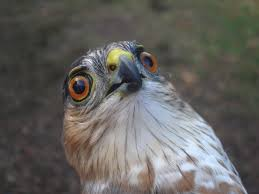
\includegraphics[width=1\linewidth]{figuras/birb_03}
			\vspace{-20pt} %Diminui espaço entre legenda e imagem
			\caption[Legenda curta do birb puto 2]{Legenda longa do birb puto 2}
			\vspace{-10pt} %Diminiui espaço vertical entre legenda e texto
			\label{fig:birb05}
			\vspace{-20pt} %Diminui espaço entre legenda e imagem
		\end{figure}
	
		Arcu dui vivamus arcu felis bibendum ut. Fames ac turpis egestas maecenas pharetra. Dolor sed viverra ipsum nunc aliquet. Arcu non odio euismod lacinia. Ut sem viverra aliquet eget. Consectetur libero id faucibus nisl tincidunt eget nullam non. Velit sed ullamcorper morbi tincidunt. Neque laoreet suspendisse interdum consectetur libero. Feugiat vivamus at augue eget arcu dictum varius. Nunc scelerisque viverra mauris in aliquam sem fringilla.

		\begin{equation} %ambiente de equações numerada
		x = \frac{-b \pm \sqrt{b^2 -4ac}}{2a}
		\end{equation}

		Magna etiam tempor orci eu lobortis elementum nibh tellus molestie. Enim lobortis scelerisque fermentum dui faucibus in ornare. Aliquam sem fringilla ut morbi tincidunt augue interdum velit. Ut lectus arcu bibendum at varius vel pharetra. Lectus mauris ultrices eros in cursus turpis massa tincidunt. Et malesuada fames ac turpis egestas maecenas pharetra. Sed cras ornare arcu dui vivamus. Accumsan sit amet nulla facilisi morbi tempus iaculis urna. Pulvinar neque laoreet suspendisse interdum consectetur libero id faucibus. Id venenatis a condimentum vitae sapien pellentesque habitant morbi. Risus sed vulputate odio ut enim. Sed euismod nisi porta lorem mollis. Elementum tempus egestas sed sed risus. Feugiat scelerisque varius morbi enim.
		\begin{table}[H] %H define 
			\centering
			\caption[Legenda curta da tabela 2]{Legenda longa da tabela 2}
			\label{tab:tab2}
			\begin{tabular}{|l|l|l|}
				\hline
				A1 & \multicolumn{2}{l|}{B1} \\ \hline %comando multicolumn para especificar quantas células mesclar {coluna}{Align |(borda)}{conteúdo}
				A2 & B2         & C2         \\ \hline
				A3 & B3         & C3         \\ \hline
			\end{tabular}
		\end{table}
		Amet consectetur adipiscing elit duis tristique sollicitudin nibh. Dignissim diam quis enim lobortis scelerisque. Lorem ipsum dolor sit amet consectetur adipiscing. At imperdiet dui accumsan sit amet nulla. Turpis egestas sed tempus urna et pharetra pharetra massa. Et netus et malesuada fames ac turpis egestas sed tempus. Porta nibh venenatis cras sed felis. Nibh sit amet commodo nulla facilisi. Varius morbi enim nunc faucibus a pellentesque sit. Leo a diam sollicitudin tempor id eu nisl nunc mi. Fermentum posuere urna nec tincidunt praesent semper feugiat nibh sed. Mi in nulla posuere sollicitudin aliquam ultrices sagittis orci a.
		
	\end{multicols}
	\newpage
	
	%%
	%%	ESTUDO NOTA RODAPÉ E CITAÇÕES
	%%
	\section{Estudo nota rodapé e citações}
		Ac turpis egestas sed tempus urna et pharetra pharetra. Sit amet nisl purus in. At quis risus sed vulputate odio ut. Placerat duis ultricies lacus sed turpis tincidunt id aliquet. Quis vel eros donec ac odio tempor orci dapibus. Sit amet mattis vulputate enim nulla aliquet porttitor lacus luctus. Ornare suspendisse sed nisi lacus sed viverra tellus. Aliquet nibh praesent tristique magna sit amet purus gravida. Risus at ultrices mi tempus. Eu sem integer vitae justo eget magna. Diam ut venenatis tellus in metus vulputate eu scelerisque felis. Nunc sed augue lacus viverra vitae. Quis eleifend quam adipiscing vitae proin. Ante in nibh mauris cursus mattis.\footnote{Esta é uma nota de rodapé} Scelerisque in dictum non consectetur a erat nam. Senectus et netus et malesuada fames ac turpis egestas. Id faucibus nisl tincidunt eget nullam. Scelerisque viverra mauris in aliquam sem fringilla ut.
	
		\subsection{Título subseção}
			Volutpat commodo sed egestas egestas fringilla phasellus. Sit amet nisl suscipit adipiscing bibendum est ultricies integer. Blandit libero volutpat sed cras ornare arcu dui vivamus arcu. Facilisis gravida neque convallis a cras semper. Venenatis a condimentum vitae sapien pellentesque habitant. Proin nibh nisl condimentum id venenatis a condimentum. Aliquam sem et tortor consequat id porta nibh. Semper feugiat nibh sed pulvinar. Mi eget mauris pharetra et. Placerat vestibulum lectus mauris ultrices eros in. Egestas egestas fringilla phasellus faucibus scelerisque eleifend donec pretium vulputate. Convallis aenean et tortor at risus. Aliquet bibendum enim facilisis gravida neque convallis a. Pharetra massa massa ultricies mi quis hendrerit dolor magna. Sapien et ligula ullamcorper malesuada proin.\footnote[516]{Esta é outra nota de rodapé com contagem zuada}
		
			\subsubsection{Título de subsubseção}
				Lorem ipsum dolor sit amet, consectetur adipiscing elit, sed do eiusmod tempor incididunt ut labore et dolore magna aliqua. Ut enim ad minim veniam, quis nostrud exercitation ullamco laboris nisi ut aliquip ex ea commodo consequat. Duis aute irure dolor in reprehenderit in voluptate velit esse cillum dolore eu fugiat nulla pariatur. Excepteur sint occaecat cupidatat non proident, sunt in culpa qui officia deserunt mollit anim id est laborum.\footnote{Esta é outra nota de rodapé hahahahaha}
			
				Lorem ipsum dolor sit amet, consectetur adipiscing elit, sed do eiusmod tempor incididunt ut labore et dolore magna aliqua. Ut enim ad minim veniam, quis nostrud exercitation ullamco laboris nisi ut aliquip ex ea commodo consequat. Duis aute irure dolor in reprehenderit in voluptate velit esse cillum dolore eu fugiat nulla pariatur.\footnote{Esta é outra nota de rodapé 1} Excepteur sint occaecat cupidatat non proident, sunt in culpa qui officia deserunt mollit anim id est laborum.\footnote{Esta é outra nota de rodapé 2}
			
		\newpage
		
	\section{Estudo citações}
		Ac turpis egestas sed tempus urna et pharetra pharetra. Sit amet nisl purus in. At quis risus sed vulputate odio ut. Placerat duis ultricies lacus sed turpis tincidunt id aliquet. Quis vel eros donec ac odio tempor orci dapibus. Sit amet mattis vulputate enim nulla aliquet porttitor lacus luctus. Ornare suspendisse sed nisi lacus sed viverra tellus. Aliquet nibh praesent tristique magna sit amet purus gravida. Risus at ultrices mi tempus. Eu sem integer vitae justo eget magna. Diam ut venenatis tellus in metus vulputate eu scelerisque felis. Nunc sed augue lacus viverra vitae. Quis eleifend quam adipiscing vitae proin. \enquote{UMA CITAÇÃO FEITA NO TEXTO.}. Scelerisque in dictum non consectetur a erat nam. Senectus et netus et malesuada fames ac turpis egestas. Id faucibus nisl tincidunt eget nullam. Scelerisque viverra mauris in aliquam sem fringilla ut. \footnote{Esta é outra nota de rodapé}
		
		\subsection{Título subseção}
			Volutpat commodo sed egestas egestas fringilla phasellus. Sit amet nisl suscipit adipiscing bibendum est ultricies integer. Blandit libero volutpat sed cras ornare arcu dui vivamus arcu. Facilisis gravida neque convallis a cras semper. Venenatis a condimentum vitae sapien pellentesque habitant. Proin nibh nisl condimentum id venenatis a condimentum. Aliquam sem et tortor consequat id porta nibh. Semper feugiat nibh sed pulvinar. Mi eget mauris pharetra et. \footnote{Esta é outra nota de rodapé com contagem NORMAL}
			
			\begin{quote}
				ESTA É UMA CITAÇÃO CURTA
			\end{quote}
			
			\begin{quotation}
				\textbf{ESTA JÁ É UMA CITAÇÃO LONGA.} Placerat vestibulum lectus mauris ultrices eros in. Egestas egestas fringilla phasellus faucibus scelerisque eleifend donec pretium vulputate. Convallis aenean et tortor at risus. Aliquet bibendum enim facilisis gravida neque convallis a. 
				
				Pharetra massa massa ultricies mi quis hendrerit dolor magna. Sapien et ligula ullamcorper malesuada proin.\footnote[516]{Esta é outra nota de rodapé com contagem zuada}
			\end{quotation}
		
			\subsubsection{Título de subsubseção}
				Lorem ipsum dolor sit amet, consectetur adipiscing elit, sed do eiusmod tempor incididunt ut labore et dolore magna aliqua. Ut enim ad minim veniam, quis nostrud exercitation ullamco laboris nisi ut aliquip ex ea commodo consequat. Duis aute irure dolor in reprehenderit in voluptate velit esse cillum dolore eu fugiat nulla pariatur. ``Excepteur sint occaecat cupidatat non proident, sunt in culpa qui officia deserunt mollit anim id est laborum."
				
				Lorem ipsum dolor sit amet, consectetur adipiscing elit, sed do eiusmod tempor incididunt ut labore et dolore magna aliqua. Ut enim ad minim veniam, quis nostrud exercitation ullamco laboris nisi ut aliquip ex ea commodo consequat. Duis aute irure dolor in reprehenderit in voluptate velit esse cillum dolore eu fugiat nulla pariatur.\footnote{Esta é outra nota de rodapé 1} Excepteur sint occaecat cupidatat non proident, sunt in culpa qui officia deserunt mollit anim id est laborum.\footnote{Esta é outra nota de rodapé 2}
				
		\newpage
	%Adciona bibliografia ao sumário
	\addcontentsline{toc}{section}{Referências} % toc (TableOfContents), section (hierarquia), Referências (nome no sumário)
	\bibliographystyle{apalike} %estilo da bibliografia e citações
	\bibliography{first_bib} %qual bibliografia adcionar as referências
	\nocite{alchemist_pauloc} %livro de referência não citado
\end{document}
		
